\documentclass[a4paper,10pt]{article}
\usepackage[utf8]{inputenc}
\usepackage{tikz}
\usepackage{amsmath}
\usepackage{fullpage}

%opening
\title{Attaque du protocole de l'équipe Trinôme du Second Degré}
\author{par l'Equipe Stone Jaws}

\begin{document}

\maketitle

\section{Le protocole}

Considérons 3 rôles $i$, $r$, et $m$ (que l'on appellera respectivement initiateur, récepteur, et serveur). La sémantique (en utilisant les notations de \cite{cas}) de ce protocole est alors donnée par :
\begin{eqnarray*}
	TdSD(i) & = & \{ (i,r,m, K, K_{im}), \\
		& & \texttt{send}_1(i,m, \textrm{senc}(\langle r,K \rangle, K_{im}) ), \\
		& & \texttt{recv}_3(r,i,  \textrm{senc}(K,K) ),\\
		& & \texttt{send}_4(i,r, h(K)) \} \\
\end{eqnarray*}
\begin{eqnarray*}
	TdSD(r) & = & \{ (i,r,m, K_{rm}), \\
		& & \texttt{recv}_2(m,r, \textrm{senc}(\langle i,V \rangle, K_{rm}) ), \\
		& & \texttt{send}_3(r,i,  \textrm{senc}(V,V) ),\\
		& & \texttt{recv}_4(i,r, h(V)) \} \\
\end{eqnarray*}
\begin{eqnarray*}
	TdSD(m) & = & \{ (i,r,m, K_{rm}, K_{im}), \\
		& & \texttt{recv}_1(i,m, \textrm{senc}(\langle r,W \rangle, K_{im}) ), \\
		& & \texttt{send}_2(m,r, \textrm{senc}(\langle i,W \rangle, K_{rm}) )  \} \\
\end{eqnarray*}




\begin{figure}
\begin{center}
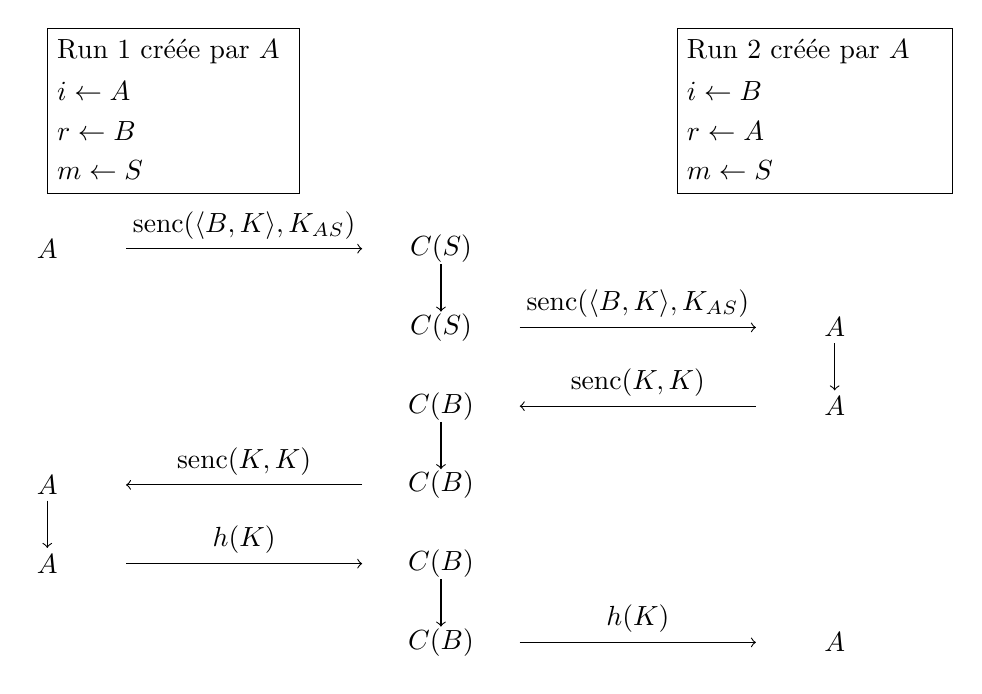
\begin{tikzpicture}
        \draw(-5,8.8) rectangle (-1.8,6.7);
	\draw (-5,8.5) node[right]{Run 1 créée par $A$};
	\draw (-5,8) node[right]{$i \leftarrow A$};
	\draw (-5,7.5) node[right]{$r \leftarrow B$};
	\draw (-5,7) node[right]{$m \leftarrow S$};
	\draw(3,8.8) rectangle (6.5,6.7);
	\draw (3,8.5) node[right]{Run 2 créée par $A$};
	\draw (3,8) node[right]{$i \leftarrow B$};
	\draw (3,7.5) node[right]{$r \leftarrow A$};
	\draw (3,7) node[right]{$m \leftarrow S$};
	\draw (-5,6) node{$A$} ;
	\draw[->]  (-4,6) -- node[above]{$\textrm{senc}(\langle B,K \rangle, K_{AS})$} (-1,6);
	\draw (0,6) node{$C(S)$} ;
	\draw[->]  (0,5.8) -- (0,5.2) ;
	\draw (0,5) node{$C(S)$} ;
	\draw[->]  (1,5) -- node[above]{$\textrm{senc}(\langle B,K \rangle, K_{AS})$} (4,5) ;
	\draw (5,5) node{$A$} ;
	\draw[->]  (5,4.8) -- (5,4.2) ;
	\draw (5,4) node{$A$} ;
	\draw[->]  (4,4) -- node[above]{$\textrm{senc}(K,K)$} (1,4) ;
	\draw (0,4) node{$C(B)$} ;
	\draw[->]  (0,3.8) -- (0,3.2) ;
	\draw (0,3) node{$C(B)$} ;
	\draw[->]  (-1,3) -- node[above]{$\textrm{senc}(K,K)$} (-4,3) ;
	\draw (-5,3) node{$A$} ;
	\draw[->]  (-5,2.8) -- (-5,2.2) ;
	\draw (-5,2) node{$A$} ;
	\draw[->]  (-4,2) -- node[above]{$h(K)$} (-1,2) ;
	\draw (0,2) node{$C(B)$};
	\draw[->]  (0,1.8) -- (0,1.2) ;
	\draw (0,1) node{$C(B)$} ;
	\draw[->]  (1,1) -- node[above]{$h(K)$} (4,1) ;
	\draw (5,1) node{$A$};
\end{tikzpicture}
\end{center}
\caption{Attaque du protocole Trinôme du Second Degré}
\label{fig1}
\end{figure}




\section{Attaque sur le protocole}
L'attaque est représentée sur la Figure \ref{fig1} et fonctionne comme suit : $A$ exécute le protocole une fois (dans la Run $1$) en tant qu'initiateur et veut s'adresser à $B$, et une autre fois (dans la Run $2$) en tant que récepteur avec $B$ dans le rôle d'initiateur. On notera $A_1$ et $A_2$ pour distinguer l'agent $A$ en tant qu'acteur des Runs $1$ et $2$.\\
\begin{enumerate}
\item $A_1$ envoie un premier message $\textrm{senc}(\langle B,K \rangle, K_{AS})$ au serveur, qui est intercepté par un agent malveillant $C$. Celui redirige exactement ce message à $A_2$, qui croit que $B$ désire communiquer avec lui. 
\item $A_2$ envoie alors à $B$ le message $\textrm{senc}(K,K)$, qui est intercepté par $C$ et le redirige vers $A_1$.
\item $A_1$ pense alors que $B$ lui a répondu, et accuse réception en lui envoyant $h(K)$, qui est intercepté par $C$ et redirigé vers $A_2$. Celui-ci croit alors que $B$ accuse réception.
\end{enumerate}

On remarque alors que deux des propriétés exigées ne sont pas vérifiées :
\begin{itemize}
\item Dans cet exemple, l'initiateur de la Run $1$ envoie un message à un récepteur et termine le protocole alors que le récepteur n'a pas reçu le message. 
\item De plus, le récepteur de la Run $2$ peut croire recevoir une donnée d'un initiateur qui ne l'a en fait jamais envoyée.
\end{itemize}

\bibliographystyle{plain}
\bibliography{ref.bib}


\end{document}
